\documentclass[12pt]{article}
\usepackage[margin=1in]{geometry}
\usepackage{amsmath,amssymb,amsthm,booktabs,graphicx,natbib,microtype}
\newtheorem{theorem}{Theorem}
\newtheorem{corollary}[theorem]{Corollary}
\newtheorem{proposition}[theorem]{Proposition}
\newtheorem{remark}[theorem]{Remark}
\newcommand{\Ran}{\operatorname{Ran}}
\newcommand{\Tr}{\operatorname{Tr}}
\newcommand{\rank}{\operatorname{rank}}
\title{Canonical Partial-Isometry Gauges\\\large Principal Angles, Changing Supports, and Minimal Positive Forcing}
\author{Prime Dynamics Theory Program}
\date{July 2026}

\begin{document}
\maketitle

\begin{abstract}
The floor-free audit RH-130 replaced positive-definite tail transport by a
semidefinite problem with rank creation, while RH-131 showed that singular
Rayleigh theory is exact on a specified support.  We now construct the
canonical gauge between changing supports.  For orthogonal projectors
$P,Q$, take the polar decomposition
\[
 QP=W|QP|.
\]
The polar factor $W$ is a basis-independent partial isometry that maps the
principal source directions to the principal target directions.  It is the
unique Procrustes optimizer when the nonzero principal cosines are simple,
and in general is the canonical optimizer selected by the polar calculus.
Its initial and final defects identify exactly which source and target
directions cannot be connected multiplicatively.

For a source tail $D$, target tail $D'$, and factor $b\geq0$, we prove that
\[
 F_b=(D'-bWDW^*)_+
\]
is a valid positive forcing and minimizes trace among all $F\succeq0$ with
$D'\preceq bWDW^*+F$.  Moreover, target mass on the complement of
$WW^*$ is an unavoidable lower bound for every such forcing.  A 4,096-case
audit verifies partial-isometry identities, Procrustes optimality against
sampled competitors, positive dominance, and the unmatched-range lower
bound with zero failures.

Applied to RH-130, the 96 adjacent pairs split canonically into 30
$0\to0$ vacuous edges, 42 $4\to4$ transport-eligible edges, and 24
$0\to4$ forcing-only edges.  The minimal normalized birth strength is
subunit on 22 of those 24 edges; the remaining two equal the previously
identified bad value $9.4363$.  The affine route is therefore neither a
formal rescue nor a uniform success: it has an exact canonical decomposition
and a sharply localized finite obstruction.
\end{abstract}

\section{Why a partial isometry is the correct gauge}
Let $E,F$ be closed subspaces of a finite-dimensional Hilbert space $H$,
with orthogonal projectors $P,Q$.  A full invertible gauge presupposes equal
dimensions and hides the possibility that a target direction has no source
ancestor.  RH-130 showed that precisely this event occurs in the discarded
memory tail: zero tail support can become four-dimensional at the next
scale.  No change of coordinates turns that birth into multiplicative
transport.

The operator $QP:E\to F$ contains all geometry shared by the two supports.
Its nonzero singular values are the principal cosines
$\cos\theta_1,\ldots,\cos\theta_k$.  Its polar factor maps the corresponding
principal vectors isometrically and leaves orthogonal or dimension-mismatched
directions unmatched.  Unlike an ordered eigenframe gauge, this construction
depends only on the two support projectors and is invariant under basis
changes inside either support \citep{Kato1995,Bhatia1997}.

\section{Canonical polar transport}
Choose orthonormal frame matrices $U$ and $V$ for $E$ and $F$.  If
\[
 V^*U=L\Sigma R^*,
\]
then the polar partial isometry is
\[
 W=V L_kR_k^*U^*,
\]
where $k$ is the number of nonzero principal cosines.  Its initial and final
projectors are
\[
 W^*W=U R_kR_k^*U^*,\qquad
 WW^*=V L_kL_k^*V^*.
\]

\begin{theorem}[Canonical principal-angle gauge]\label{thm:polar}
The operator $W$ is the polar factor of $QP$.  It is independent of the
chosen frames $U,V$, maps paired principal source vectors to paired target
vectors, and has rank $k=\rank(QP)$.  Among rank-$k$ partial isometries with
initial space in $E$ and final space in $F$, it maximizes
\[
 \Re\Tr(X^*QP)=\sum_{j=1}^k\cos\theta_j.
\]
For equal-dimensional transverse supports it equivalently minimizes the
orthogonal Procrustes displacement between their frames.
\end{theorem}

\begin{proof}
The displayed singular-value decomposition gives
$QP=VL\Sigma R^*U^*$ on $E$, hence its polar decomposition has partial
factor $V L_kR_k^*U^*$.  Replacing $U,V$ by different orthonormal frames
conjugates the reduced factors and leaves the ambient operator unchanged.
Von Neumann's trace inequality bounds the objective for every admissible
$X$ by the sum of the first $k$ singular values of $QP$; the polar factor
attains equality.  In the equal-rank case,
$\|VO-U\|_F^2=2r-2\Re\Tr(O^*V^*U)$, so the same maximizer solves the
Procrustes problem \citep{GolubVanLoan2013}.
\end{proof}

The theorem gives a natural geometry-only gauge, but it does not yet make
the gauge dynamical: a future paper must show that the memory/packet update
actually produces these adjacent support projectors or a controlled
approximation to them.

\section{Unmatched directions are forcing}
Let $D\succeq0$ be supported on $E$, let $D'\succeq0$ be supported on $F$,
and set $\widetilde D=WDW^*$.  Fix a proposed multiplicative factor $b$.
The Hermitian residual is
\[
 X_b=D'-b\widetilde D.
\]
Write $X_b=X_{b,+}-X_{b,-}$ for its positive and negative parts.

\begin{theorem}[Trace-minimal positive forcing]\label{thm:forcing}
The operator
\[
 F_b=X_{b,+}
\]
satisfies $F_b\succeq0$ and
$D'\preceq b\widetilde D+F_b$.  Among all positive $F$ satisfying this
inequality, it has minimum trace:
\[
 \Tr F\geq\Tr X_{b,+}=\Tr F_b.
\]
\end{theorem}

\begin{proof}
Since $F_b-X_b=X_{b,-}\succeq0$, the displayed forcing is feasible.  Let
$P_+$ be the positive spectral projector of $X_b$.  For any feasible
$F$, compression of $F-X_b\succeq0$ to $P_+H$ gives
$\Tr(P_+FP_+)\geq\Tr X_{b,+}$.  Positivity gives
$\Tr F\geq\Tr(P_+FP_+)$, proving optimality.
\end{proof}

This result does not claim that $F_b$ is the least element in Loewner order;
positive majorants need not form a lattice.  Trace is the exact convex cost
for which the positive part is canonical and sharp.

\begin{corollary}[Unmatched target lower bound]\label{cor:unmatched}
Let $Q_0=I-WW^*$ be the unmatched target projector.  Every feasible forcing
satisfies
\[
 Q_0FQ_0\succeq Q_0D'Q_0,
 \qquad
 \Tr F\geq\Tr(Q_0D'Q_0).
\]
\end{corollary}
\begin{proof}
The transported tail is supported on $WW^*$, so
$Q_0\widetilde DQ_0=0$.  Compress the defining inequality to $Q_0H$ and
take traces.
\end{proof}

Thus a target dimension excess is not just a poor principal angle.  It is
an additive source with a quantitative, gauge-independent lower bound.
When $D=0$ and $D'\neq0$, the whole target tail is forcing and
$F_b=D'$ for every $b$.

\section{Synthetic audit}
We sample 4,096 pairs of subspaces in ambient dimension twelve.  Half have
equal ranks one through six; half have target rank strictly larger than
source rank.  In every case the SVD polar map satisfies its initial and
final projector identities.  On the 2,048 equal-rank cases, it beats all 48
random orthogonal Procrustes competitors sampled per instance.  Random
positive source and target tails then test Theorem~\ref{thm:forcing}: every
positive-part forcing dominates the residual, and its trace exceeds the
unmatched target lower bound.  No failure occurs.  The tests are numerical
checks of exact finite-dimensional theorems, not evidence for all-level
dynamical coherence.

\begin{figure}[t]
\centering
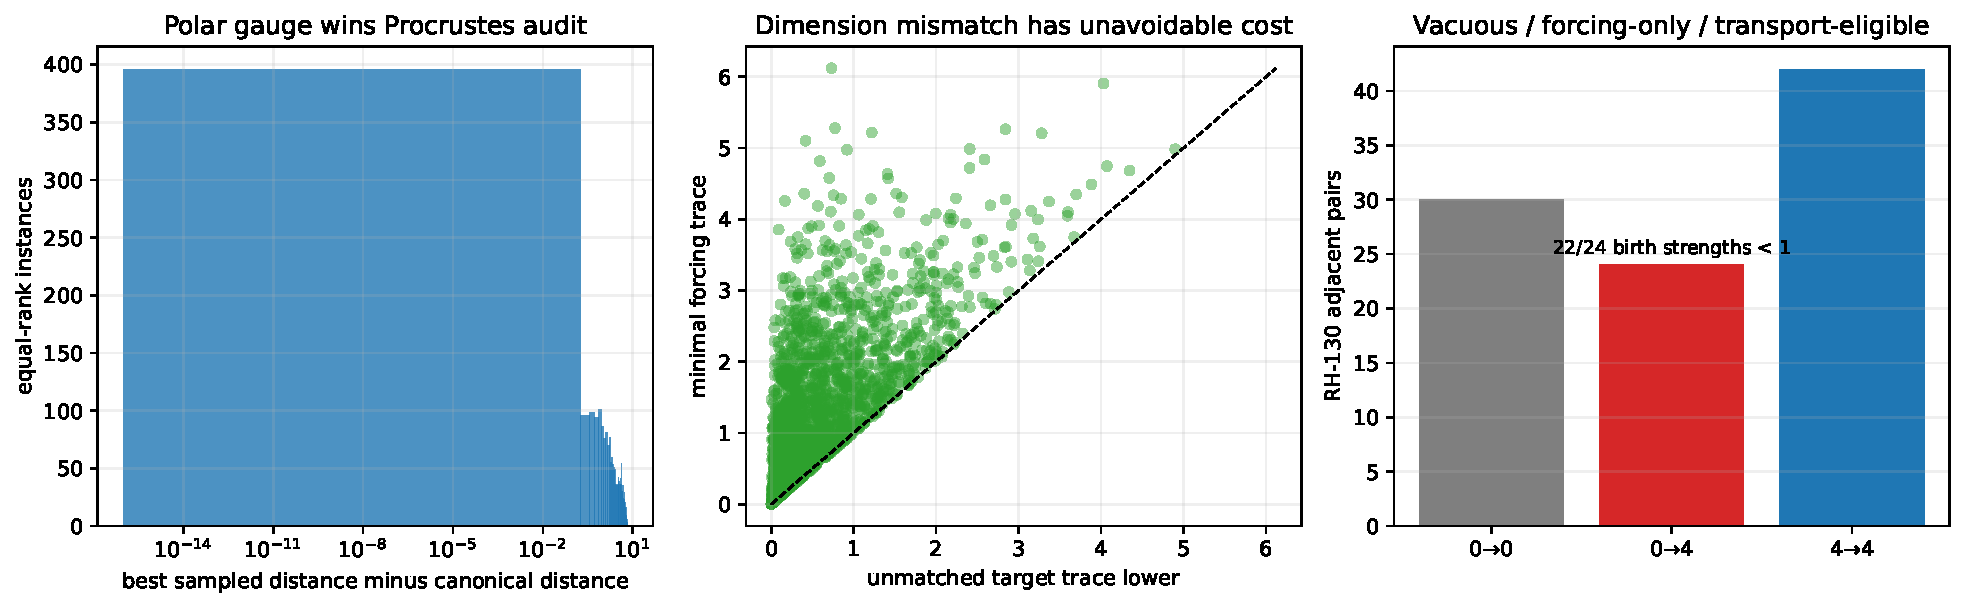
\includegraphics[width=\textwidth]{figures/canonical_partial_isometry_forcing_gauge.pdf}
\caption{Procrustes advantage of the polar gauge, unavoidable unmatched
forcing, and the exact RH-130 transition classification.}
\label{fig:audit}
\end{figure}

\section{RH-130 decomposition and affine implications}
The 120 RH-130 states have tail rank either zero or four.  Pairing adjacent
scales, 30 edges are $0\to0$, 42 are $4\to4$, and 24 are $0\to4$; there are
no $4\to0$ edges.  The polar-gauge interpretation is immediate.

On a $0\to0$ edge, tail transport is vacuous.  On a $4\to4$ edge, the full
reduced support is transport-eligible; 37 of these 42 edges give a positive
floor-free multiplicative candidate, while five have a finite factor but
push the transferred Rayleigh constant to at least one.  On every
$0\to4$ edge, the source tail is zero and the target tail is entirely a
birth term.  The infinite factors of RH-130 are exactly these 24 cases.

In normalized target coordinates the least scalar forcing for a birth edge
is its target squared Rayleigh constant.  Across the 24 births this value
ranges from $6.19\times10^{-24}$ to $9.4363$, with median
$1.51\times10^{-12}$.  Twenty-two births are subunit.  The two superunit
births are the left-channel final-phase states at $\sigma=0.08$ already
isolated in RH-130.  Hence additive forcing repairs the rank logic on every
edge, but does not automatically restore positivity on those two states.

The next task is no longer ambiguous.  One must derive adjacent supports and
their polar map from the actual packet recursion, decompose the next tail as
transported old tail plus a born-memory block, and estimate the normalized
trace or Rayleigh cost of that block.  Post hoc optimization over arbitrary
exact-Gram gauges is no longer the target.

We have constructed a canonical support gauge, proved its principal-angle
optimality, and identified the trace-minimal positive forcing and unmatched
lower bound.  We have not derived this gauge from the physical memory
recursion, proved all-level affine coefficients, controlled the two finite
superunit birth states, established a normalized-base liminf or uniform
Stage A, constructed a Hilbert--Polya operator, identified zeta zeros, or
proved the Riemann Hypothesis.

\bibliographystyle{plainnat}
\bibliography{references}
\end{document}
